\chapter{Equipments}

In this project, necessary equipments, software, and robotic arm that are going to be used are: 1 $\times$ Denso VS060A3-AV6 arm, 1 $\times$ end-effector handle, 1 $\times$ ATI Gamma F/T Sensor (SI-32-2.5 calibration), Ubuntu 12.04 LTS, OpenRave, and Denso ROS. 

\section{Denso VS060}
Denso VS060A3-AV6 is a six DOF robotic arm from Denso company. It has absolute encoder for all of its joint position.  An RC-8 controller is also provided for interfacing with this arm. The computer is connected to Denso arm via LAN cable. The architecture of the hardware interface for this arm can be seen in figure below.
\begin{figure}[H]
  \begin{subfigure}[t]{0.5\textwidth}
    \centering
    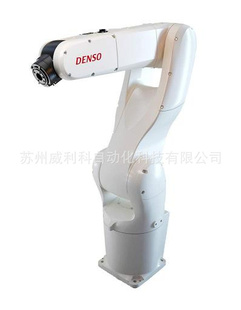
\includegraphics[width = 0.7\textwidth ]{denso_vs} 
    \caption{Denso VS060 arm}
    \label{fig:Denso arm}}
  \end{subfigure}
  \begin{subfigure}[t]{0.5\textwidth}
    \centering
    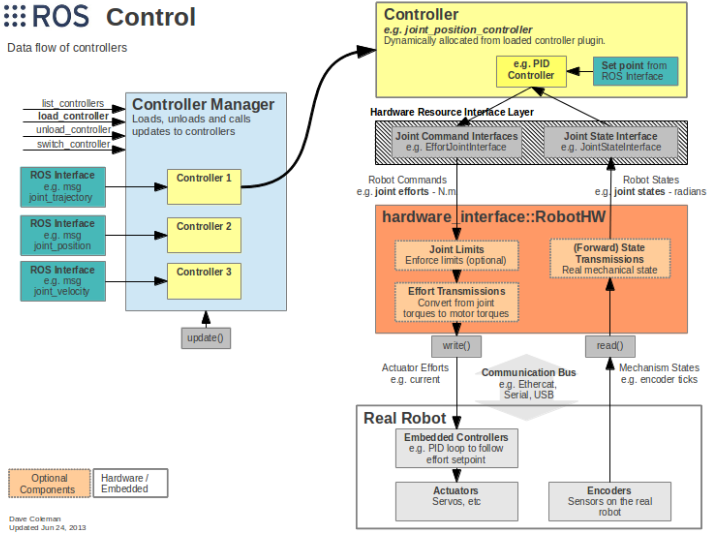
\includegraphics[width = \textwidth ]{hardware_interface}
    \caption{Hardware interface of Denso arm}
    \label{fig:hardware interface}
  \end{subfigure}
  \caption{Denso VS060A3-AV6}
\end{figure}

\section{ATI Gamma F/T Sensor}
ATI Gamma F/T sensor SI-32-2.5 is used for the experiment. It has been calibrated with the following sensing range: $ f = [32, 32, 100] N $ and $\tau = [2.5, 2.5, 2.5] Nm$. This F/T Sensor is attached into the end-effector of Denso arm to measure the contact force and torque. After this sensor, another handle is attached on top of the F/T sensor. Hence, with the addition of contact force and torque, F/T sensor will also read the weight and inertial force from the handle. 
\begin{figure}[H]
    \centering
    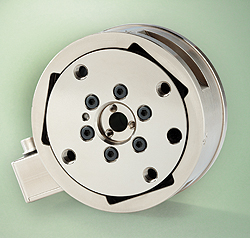
\includegraphics[width = 0.4\textwidth ]{gamma_sensor}
    \caption{ATI Gamma F/T Sensor}
    \label{fig:F/T sensor}
\end{figure}

\section{End-effector handle}
This is the handle of the end-effector arm. It has a round sphere surface. The arm will make a contact with environments through this handle.
\begin{figure}[H]
    \centering
    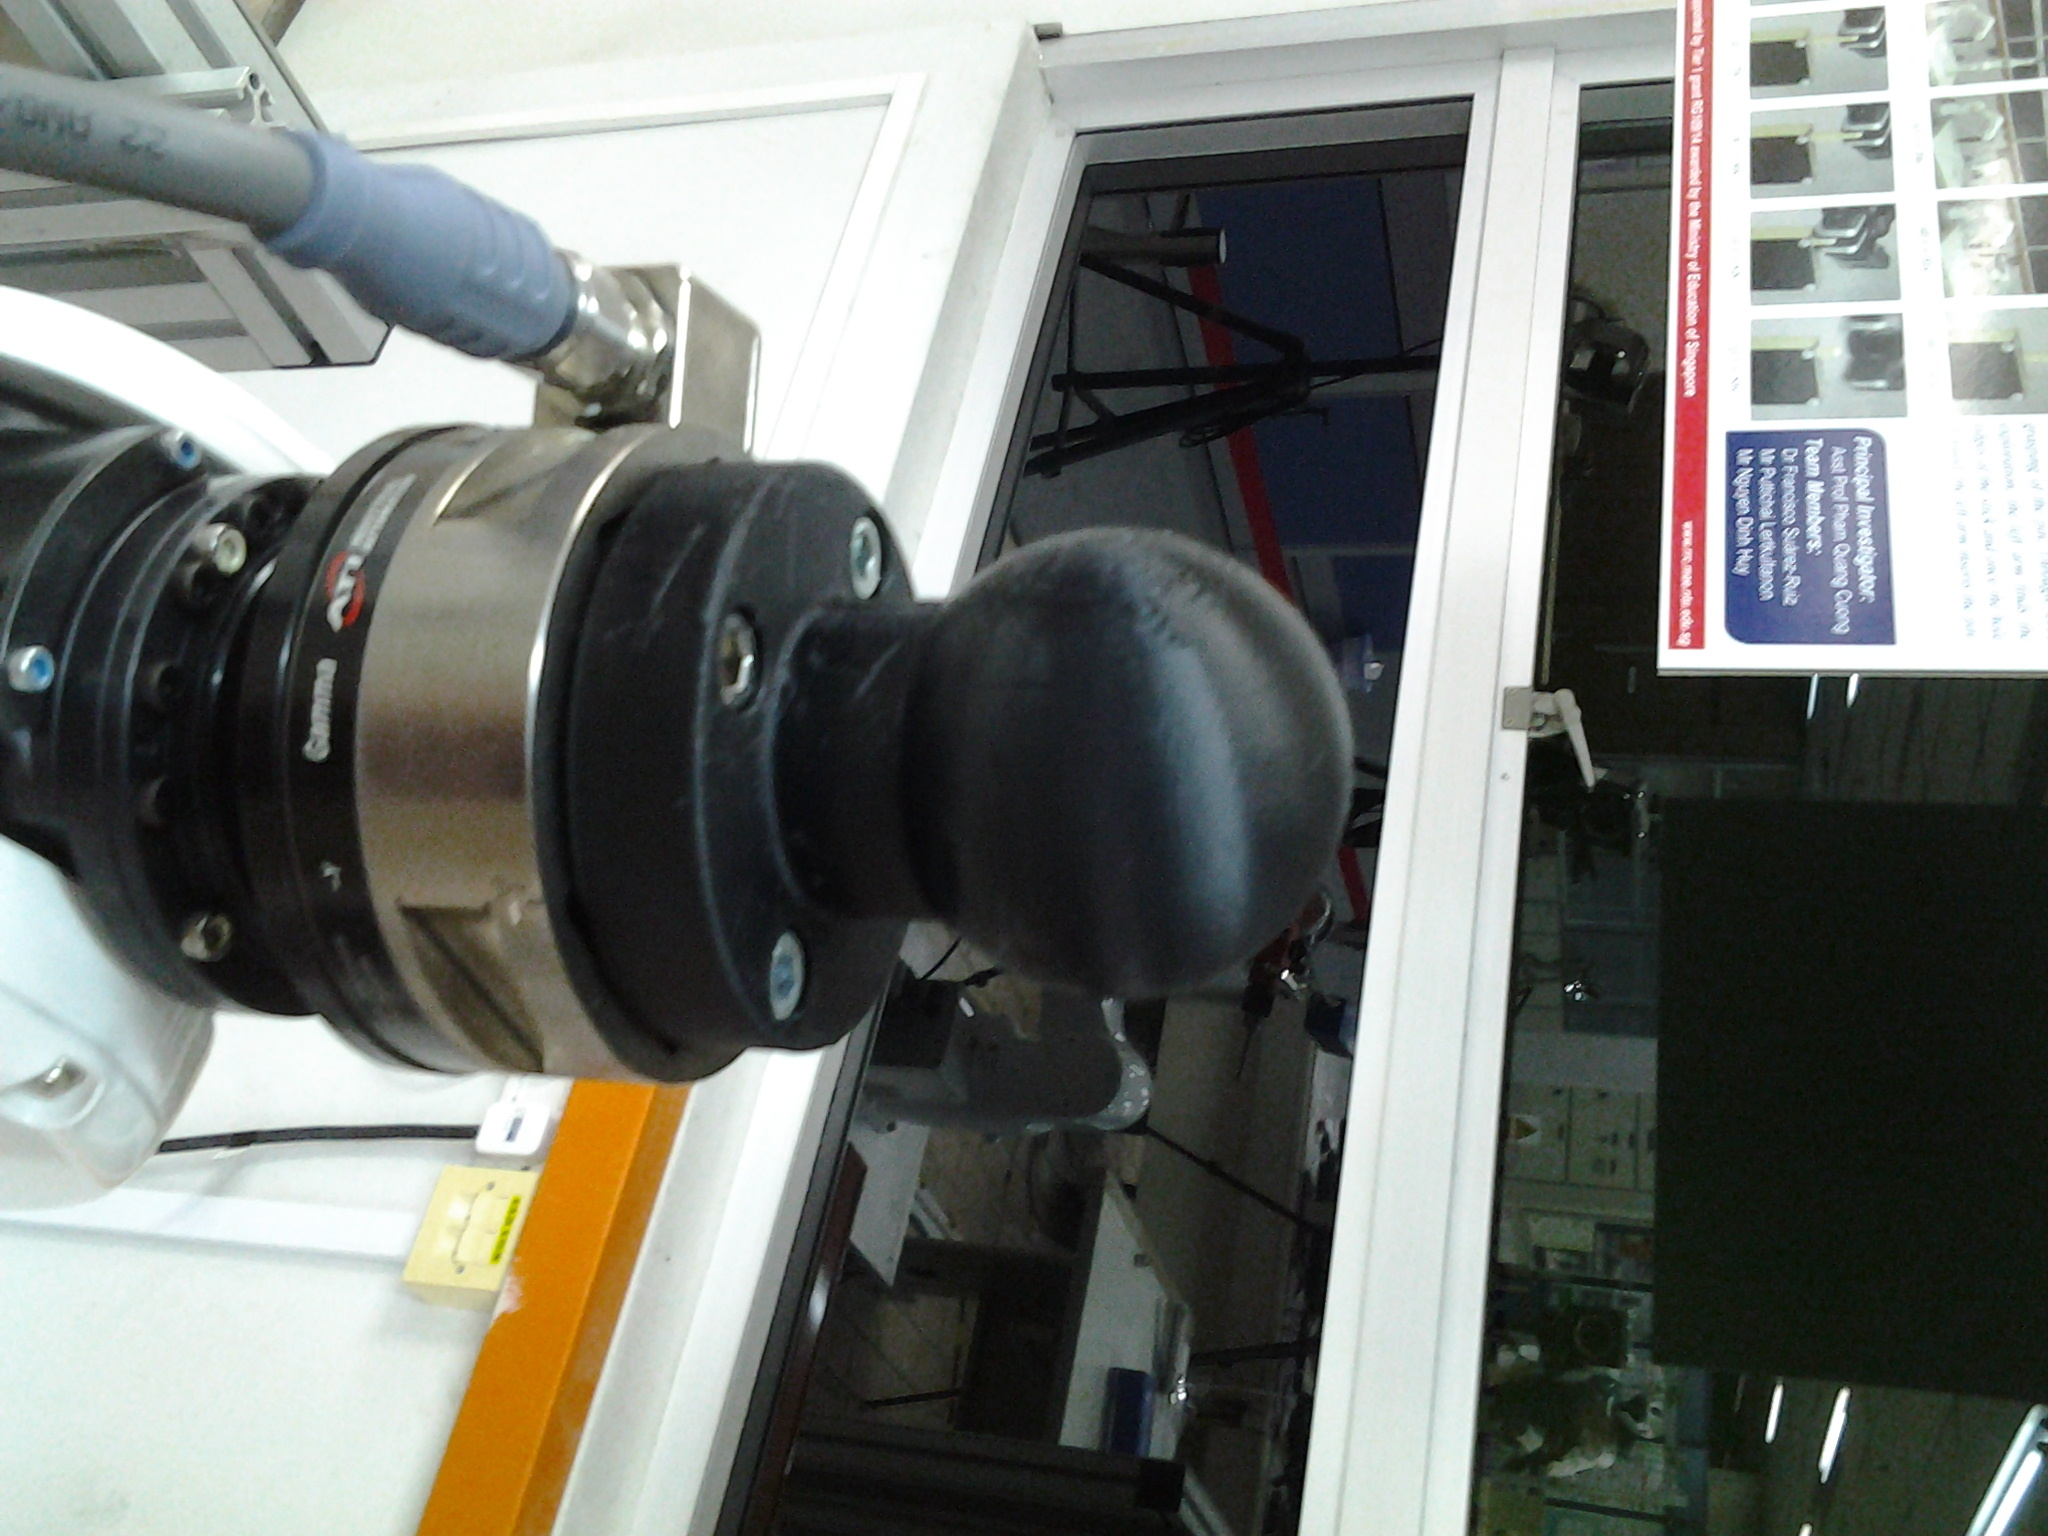
\includegraphics[width = 0.4\textwidth , angle = 90]{handle}
    \caption{End-effector handle}
    \label{fig:end-effector}
\end{figure}

\section{Ubuntu 12.04 LTS}
The OS of the working computer is Linux Ubuntu, with version of 12.04. It is not the lattest version and it should stay in 12.04 version for operating the arm. Some important packages are also installed, they are OpenRave and Denso ROS. Python and C++ are used to run the Denso arm.

\section{OpenRave}
OpenRAVE is a package that provides an environment for testing, developing, and deploying motion planning algorithms in robotics applications. It focuses on the simulation analysis of motion planning. It is to be used together with Denso ROS to control the Denso arm with its analysis guidance. The OpenRave is oftenly used in Python script.
\begin{figure}[H]
    \centering
    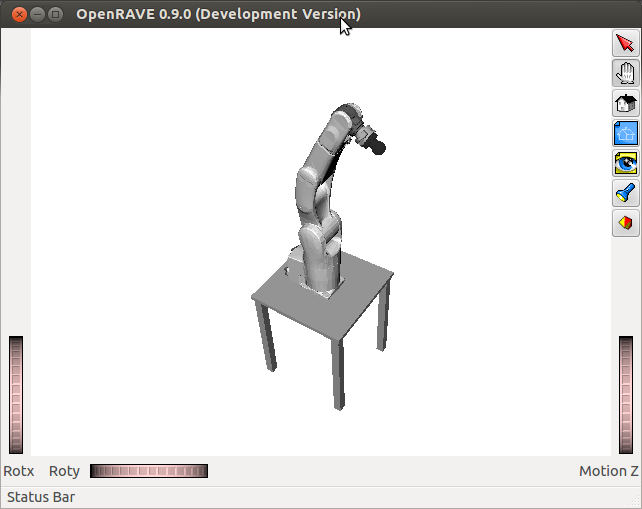
\includegraphics[width = 0.6\textwidth ]{openrave}
    \caption{OpenRave environment}
    \label{fig:OpenRave}
\end{figure}
  
\section{Denso ROS}
Denso ROS is a robot operating system that works on the Denso arm. With Denso ROS, the manipulator arm can be controlled from computer. The packages are written in C++ and Python while the script to run the robot is usually written in Python codes.
